% =====================================================================
\section{Preliminaries}\label{ch:prelim}
% =====================================================================

Vector calculus combines the two objects studied in the previous reviewers:
\emph{vector functions} $\vr(t)$, which describe curves (No.~5), and
\emph{gradients} $\grad f$, which describe how a scalar function changes
(No.~6). This chapter recalls exactly the facts that will be used.

\subsection{Gradients}

For $f(x,y)$ and $f(x,y,z)$,
\[
  \grad f=\ip{f_x,f_y}=f_x\vi+f_y\vj,\qquad
  \grad f=\ip{f_x,f_y,f_z}=f_x\vi+f_y\vj+f_z\vk .
\]
$\grad f$ points in the direction of fastest increase of $f$, has length equal
to that maximal rate, and is perpendicular to the level curves (surfaces) of
$f$.

\subsection{Curves, tangent vectors and arc length}

A (smooth) curve $C$ is described by a vector function
\[
  \vr(t)=\ip{x(t),y(t)}\quad\text{or}\quad\vr(t)=\ip{x(t),y(t),z(t)},\qquad a\le t\le b,
\]
with $\vr\,'(t)$ continuous and never $\vzero$. As $t$ increases from $a$ to $b$
the point moves from the \emph{initial point} $\vr(a)$ to the \emph{terminal
point} $\vr(b)$; this gives $C$ an \emph{orientation}.
\begin{itemize}
  \item $\vr\,'(t)$ is tangent to $C$ and points in the direction of motion.
  \item The \emph{speed} is $\norm{\vr\,'(t)}$, and the arc length element is
        $\dd s=\norm{\vr\,'(t)}\,\dd t$, so the length of $C$ is
        $L=\int_a^b\norm{\vr\,'(t)}\,\dd t$.
\end{itemize}

\begin{strategy}{Standard parametrizations (memorize).}
\begin{itemize}
  \item Segment from $P_0$ to $P_1$: $\;\vr(t)=(1-t)\vr_0+t\vr_1=\vr_0+t(\vr_1-\vr_0)$, $0\le t\le1$.
  \item Circle $x^2+y^2=R^2$, counterclockwise: $\;\vr(t)=\ip{R\cos t,R\sin t}$, $0\le t\le2\pi$.
  \item Graph $y=g(x)$, $a\le x\le b$: $\;\vr(t)=\ip{t,g(t)}$, $a\le t\le b$.
  \item Graph $x=h(y)$: $\;\vr(t)=\ip{h(t),t}$.
  \item Helix: $\;\vr(t)=\ip{\cos t,\sin t,t}$.
\end{itemize}
\end{strategy}

\begin{example}\label{ex:prelim-seg}
Parametrize the segment from $(2,0,0)$ to $(3,4,5)$ and find its length.
\end{example}
\begin{solution}
$\vr(t)=\ip{2,0,0}+t\ip{1,4,5}=\ip{2+t,\,4t,\,5t}$, $0\le t\le1$. Then
$\vr\,'(t)=\ip{1,4,5}$, $\norm{\vr\,'(t)}=\sqrt{42}$, and $L=\int_0^1\sqrt{42}\,\dd t=\sqrt{42}$
(which is, of course, the distance between the two points).
\end{solution}

\subsection{Equality of mixed partial derivatives}

The test for conservative vector fields in Chapter~\ref{ch:conservative} rests
on the following theorem.

\begin{theorem}[Clairaut]\label{thm:clairaut}
If $f$ is defined on an open disk containing $(a,b)$ and $f_{xy}$, $f_{yx}$ are
both continuous there, then $f_{xy}(a,b)=f_{yx}(a,b)$. The same holds for
functions of three variables and any pair of variables.
\end{theorem}

\begin{example}\label{ex:clairaut}
Verify Clairaut's theorem for $f(x,y)=x^3y^2+e^{xy}$.
\end{example}
\begin{solution}
$f_x=3x^2y^2+ye^{xy}$, so $f_{xy}=(f_x)_y=6x^2y+e^{xy}+xye^{xy}$.\\
$f_y=2x^3y+xe^{xy}$, so $f_{yx}=(f_y)_x=6x^2y+e^{xy}+xye^{xy}$. They agree.\checkok
\end{solution}

\subsection{Partial integration}

To recover a function from one of its partial derivatives we integrate with
respect to one variable while holding the others fixed. Because anything that
does not depend on the integration variable differentiates to zero, the
``constant of integration'' is an arbitrary \emph{function of the other
variables}.

\begin{example}\label{ex:partial-int}
Find all functions $f(x,y)$ with $f_x=2xy+y^3$.
\end{example}
\begin{solution}
Integrate with respect to $x$, treating $y$ as a constant:
\[
  f(x,y)=\int(2xy+y^3)\,\dd x=x^2y+xy^3+g(y),
\]
where $g$ is an arbitrary differentiable function of $y$ alone. Check:
$\pd{}{x}\big(x^2y+xy^3+g(y)\big)=2xy+y^3+0$.\checkok
\end{solution}

\begin{warning}
Writing ``$+C$'' instead of ``$+g(y)$'' here is a serious error: it throws
away information that is needed in the next step of the potential-function
method (Section~\ref{sec:potential}).
\end{warning}

\subsection{Types of regions}

\begin{itemize}
  \item A region $D$ is \emph{open} if around each of its points there is a
        small disk (ball) contained in $D$; e.g. an open disk, the whole plane,
        the plane minus a point.
  \item $D$ is \emph{connected} if any two points of $D$ can be joined by a
        path lying in $D$.
  \item A connected region in the plane is \emph{simply connected} if every
        simple closed curve in $D$ encloses only points of $D$; informally,
        $D$ has no holes. A disk, a half-plane and $\R^2$ are simply connected;
        an annulus and the punctured plane $\R^2\setminus\{(0,0)\}$ are not.
        (In space, $\R^3$ with a single point removed \emph{is} simply
        connected, while $\R^3$ minus a whole line is not.)
\end{itemize}

\begin{figure}[H]
\centering
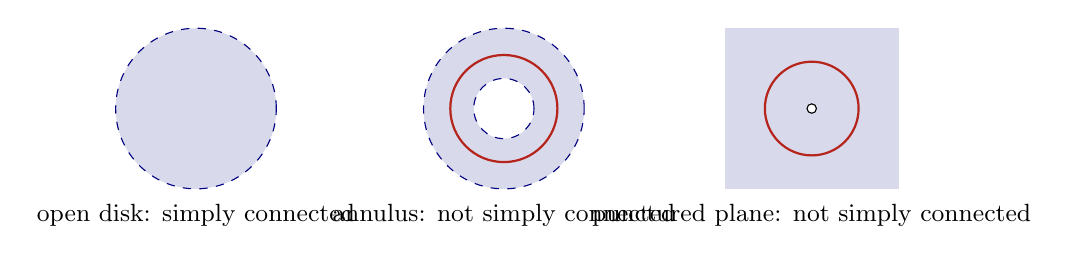
\begin{tikzpicture}[scale=0.85]
  \begin{scope}
    \fill[NavyBlue!15] (0,0) circle (1.2);
    \draw[NavyBlue,dashed] (0,0) circle (1.2);
    \node at (0,-1.6) {\small open disk: simply connected};
  \end{scope}
  \begin{scope}[xshift=4.6cm]
    \fill[NavyBlue!15, even odd rule] (0,0) circle (1.2) (0,0) circle (0.45);
    \draw[NavyBlue,dashed] (0,0) circle (1.2);
    \draw[NavyBlue,dashed] (0,0) circle (0.45);
    \draw[BrickRed,thick] (0,0) circle (0.8);
    \node at (0,-1.6) {\small annulus: not simply connected};
  \end{scope}
  \begin{scope}[xshift=9.2cm]
    \fill[NavyBlue!15] (-1.3,-1.2) rectangle (1.3,1.2);
    \filldraw[fill=white,draw=black] (0,0) circle (2pt);
    \draw[BrickRed,thick] (0,0) circle (0.7);
    \node at (0,-1.6) {\small punctured plane: not simply connected};
  \end{scope}
\end{tikzpicture}
\caption{The red loops in the middle and right pictures surround points that
are not in the region; they cannot be shrunk to a point inside the region.}
\label{fig:regions}
\end{figure}

These words matter because the component test for conservative fields
(Theorems~\ref{thm:test2} and~\ref{thm:test3}) is only guaranteed on
simply connected regions, such as the open disks and open balls named in the
slides; see Section~\ref{sec:caveat}.
